\newcommand{\figureMusicWeWillRockYouSimplified}[1]{
  \def\lang{\detokenize{#1}}
  \def\langRu{\detokenize{ru}}
  \def\langEn{en}
  \def\figureCaption{XXX: No translation.}
  \ifx \lang\langRu
  \def\figureHzUnit{Гц}
  \def\figureCaption{
    Ритм мелодии ``We Will Rock You'' группы Queen (упрощенная версия.)
  }
  \fi
  \if \lang\langEn
  \def\figureHzUnit{Hz}
  \def\figureCaption{
    The rhythm of the melody ``We Will Rock You'' by Queen (simplified
    version.)
  }
  \fi
  \begin{figure}[ht]
    \centering
    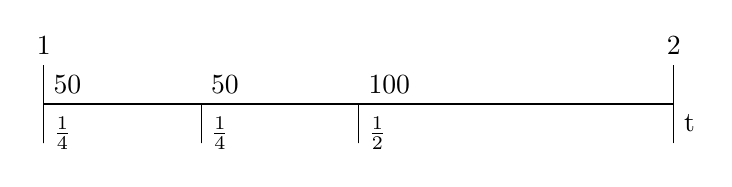
\begin{tikzpicture}
      \draw[thick] (0, 0.5) -- (8, 0.5) node[anchor=north west] {t};
      \foreach \x/\n in {0/1, 8/2} {
        \draw (\x, 0) -- (\x, 1) -- (\x, 1) node[midway, above] {\n};
      };

      \foreach \x in {0, 2} {
        \draw (\x, 0) -- (\x, 0.5) node[pos=0.25, right] {$ \frac{1}{4} $};
      };

      \draw (4, 0) -- (4, 0.5) node[pos=0.25, right] {$ \frac{1}{2} $};

      \foreach \x/\freq in {0/50, 2/50} {
        \draw (\x, 0) -- (\x, 0.5) node[pos=1.5, right] {\freq \figureHzUnit};
      };
      \draw (4, 0) -- (4, 0.5) node[pos=1.5, right] {100 \figureHzUnit};
    \end{tikzpicture}
    \caption{\figureCaption}
    \label{fig:queen-we-will-rock-you-rhythm-1}
  \end{figure}
}
